% Spring 基础篇
% 
% zzy.hit@gmail.com
% 2013/05/24

\documentclass[xcolor=dvipsnames]{beamer}
\usetheme{Warsaw}
\setbeamertemplate{items}[circle]
\definecolor{links}{HTML}{2A1B81}
\hypersetup{colorlinks,linkcolor=,urlcolor=links}
\usepackage{CJKutf8}
\usepackage{verbatim}

\title{Introduction to Spring}
\subtitle{Inversion of Control and Aspect Oriented Programming}
\author{zzy.hit@gmail.com}
\date{\today}

\begin{document}
\begin{CJK}{UTF8}{gkai}


  % title page 
  \frame{\titlepage}

  % outline
  \frame{\frametitle{内容}
    \begin{itemize}
    \item IoC - Inversion of Control
    \item Spring简介
    \item Spring入门
    \item AOP - Aspect-Oriented Programming
    \end{itemize}
  }

  \frame{\frametitle{目标}
    \begin{itemize}
    \item 理解IoC
    \item 能够正确处理类的依赖关系
    \item 能够使用xml和annotation装配应用
    \item 理解AOP原理
    \end{itemize}
  }

  % IoC
  \frame{
    \begin{center}
      IoC - Inversion of Control
    \end{center}
  }

  \frame{\frametitle{IoC (Inversion of Control)}
    \begin{block}{定律一}
      高层不应依赖低层,模块都必须抽象
    \end{block}
    \verbatiminput{../ioc1.c}
    \pause
    \textcolor{red}{now, save to database?}
    \pause
    \begin{itemize}
    \item 高层逻辑通常是抽象业务,应该具有可重用性
    \item 不应依赖底层某个模块实现
    \end{itemize}
  }

  \frame{\frametitle{IoC (Inversion of Control)}
    \begin{block}{定律二}
      实现必须依赖抽象,而不是抽象依赖实现
    \end{block}
    \verbatiminput{../ioc2_1.java}
    \pause
    \textcolor{red}{now, save to database?}
  }

  \frame{\frametitle{IoC (Inversion of Control)}
    \verbatiminput{../ioc2_2.java}
    \pause
    \textcolor{red}{FileWriter? DatabaseWriter? NetWriter? CompositeWriter...}
  }

  \frame{\frametitle{Ioc (Inversion of Control)}
    \begin{center}
      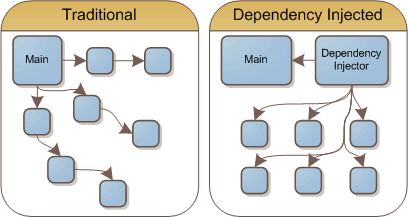
\includegraphics[width=0.8\textwidth]{../inversion-of-control.png}
    \end{center}
  }

  \frame{\frametitle{IoC (Inversion of Control)}
    
    \begin{block}{定律三}
      应用不应依赖容器,容器应服务于应用
    \end{block}

    \begin{itemize}
    \item 业务逻辑不做修改可迁移
    \item 容器不侵入应用
    \end{itemize}

    \begin{center}
      
\includegraphics[width=0.3\textwidth]{../spring_logo_mini.png}
      
\includegraphics[width=0.3\textwidth]{../pico_container_logo.png}

      
\includegraphics[width=0.3\textwidth]{../seasar_logo_blue.png}
      
\includegraphics[width=0.3\textwidth]{../guice_logo.png}
    \end{center}
  }

  % uncle bob
  \frame{\frametitle{Questions?}
    \begin{center}
      
\includegraphics[width=0.8\textwidth]{../uncle_bob.jpg}

      \href{http://www.objectmentor.com/resources/articles/dip.pdf}{The Dependency Inversion Principle} - Uncle Bob

    \end{center}
  }

  % Sample
  \frame{\frametitle{举个例子}
    \begin{center}
      
\includegraphics[width=0.8\textwidth]{../sample.jpg}
    \end{center}
  }

  % spring
  \frame{
    \begin{center}
      
\includegraphics[width=0.5\textwidth]{../spring_logo.png}
    \end{center}
  }

  \frame{\frametitle{Spring简介}
    Spring的核心是一个轻量级的IoC (Inversion of Control) 容器。用它构建的应用可以达到模块间低耦合,可测试,最终使得整个系统结构简化,易于维护。

    \begin{itemize}
    \item 轻量级(Lightweight)

      体积小(核心不足1M)、资源少、无侵入(Nonintrusive)
    \item 容器(Container)

      管理组件生命周期、状态、依赖关系等
    \item IoC (Inversion of Control)

      通过配置维护组件依赖关系,无需编码
    \end{itemize}
  }

  \frame{\frametitle{Spring简介}
    除此之外,Spring的目标是实现一个全方位的整合框架,其下由多个子框架组合,子框架之间彼此独立,并可以使用其他框架方案代替。

    \begin{itemize}
    \item AOP框架

      Spring神器之一(Aspect-Oriented Programming)
    \item 持久层

      如JDBC、ORM(Hibernate、iBatis)、事务处理等
    \item Web框架

      Spring提供了自己的Web框架,同时你也可以用其他框架来代替,如Struts、Webwork等
    \end{itemize}
  }

  \frame{\frametitle{Spring Framework}
    \begin{center}
      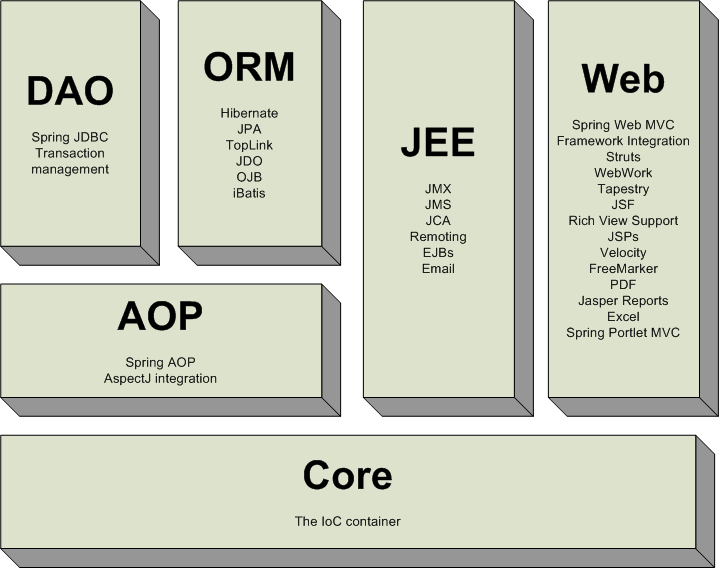
\includegraphics[width=0.9\textwidth]{../spring_framework.png}
    \end{center}
  }

  \frame{\frametitle{工作方式}
    \begin{center}
      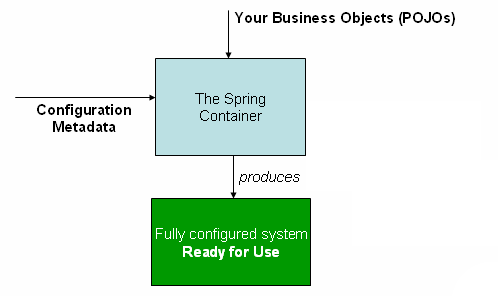
\includegraphics[width=0.8\textwidth]{../spring_container.png}
    \end{center}
  }

  % Pack app using Spring
  \frame{\frametitle{配置 - Bean定义}
    \begin{itemize}
    \item id/name, class
    \item constructor-arg, properties, value/ref/value-ref
    \item abstract/parent
    \end{itemize}
  }

  % factory/builder
  \frame{\frametitle{BeanFactory}
    \begin{itemize}
    \item getBean(String):Object
    \item getBean(String, Class):T
    \item getBean(Class):T
    \item getBean(String, Object...):Object
    \item containsBean(String):boolean
    \item isSingleton(String):boolean
    \item isPrototype(String):boolean
    \item isTypeMatch(String, Class):boolean
    \item getType(String):Class
    \item getAliases(String):String[]
    \end{itemize}
  }

  % 
  \frame{\frametitle{LifeCycle}
    \begin{itemize}
    \item init-method - InitializingBean
    \item destroy-method - DisposableBean
    \item lazy-init
    \end{itemize}
  }

  \frame{\frametitle{FactoryBean}
    \begin{itemize}
    \item getObject():T
    \item getObjectType():Class
    \item isSingleton():boolean
    \item factory-bean / factory-method
    \end{itemize}
  }

  \frame{\frametitle{Scope}
    scope(sigleton/prototype/request/session/global)
  }

  % (util:list/map/properties)

  \frame{\frametitle{ApplicationContext}
    \begin{center}
      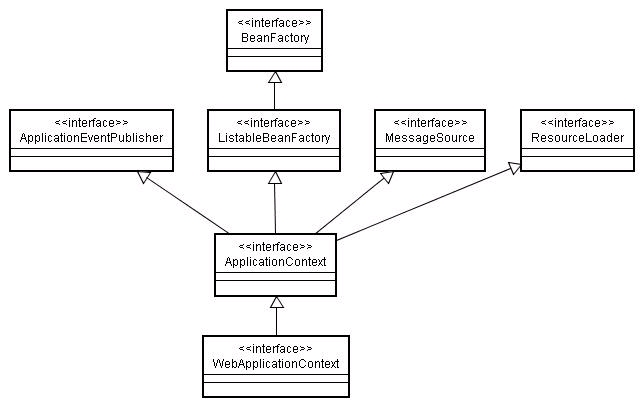
\includegraphics[width=1.0\textwidth]{../beanfactory.jpg}
    \end{center}
  }

  \frame{\frametitle{Annotation - 代码即配置}
    \begin{itemize}
    \item what is annotation
    \item @Service
      \begin{itemize}
      \item value:String
      \end{itemize}
    \item @Resource(Autowired)
      \begin{itemize}
      \item name:String
      \item type:Class
      \end{itemize}
    \item xml vs annotation
    \end{itemize}
  }

  % AOP
  \frame{
    \begin{center}
      AOP - Aspect Oriented Programming
    \end{center}
  }

  \frame{\frametitle{AOP原理}
    \verbatiminput{../aop-pojo.java}
  }

  \frame{\frametitle{AOP原理-直接调用}
    \verbatiminput{../aop-pojo-call.java}

    \begin{center}
      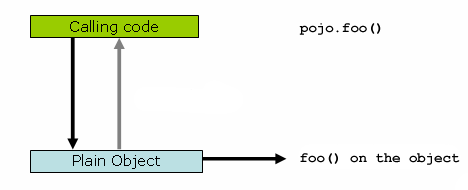
\includegraphics[width=0.7\textwidth]{../aop-proxy-plain-pojo-call.png}
    \end{center}
  }

  \frame{\frametitle{AOP原理-Proxy调用}
    \verbatiminput{../aop-pojo-proxy-call.java}

    \begin{center}
      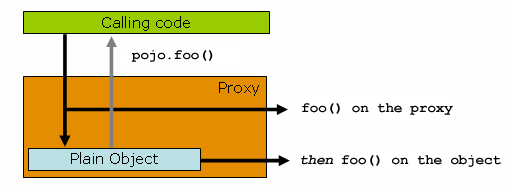
\includegraphics[width=0.7\textwidth]{../aop-proxy-call.png}
    \end{center}
  }

  \frame{\frametitle{AOP原理}
    \verbatiminput{../aop-conf.xml}
    \begin{itemize}
      \item 在哪里执行
      \item 执行什么
    \end {itemize}
  }

  \frame{\frametitle{使用场景}
    \begin{center}
      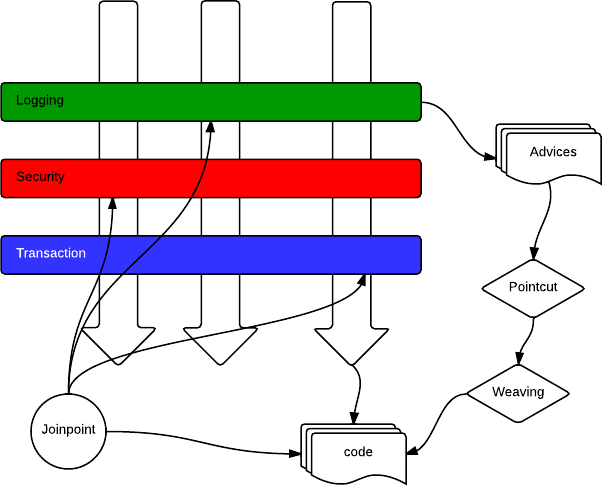
\includegraphics[width=0.8\textwidth]{../aop-usage.png}
    \end{center}
  }


  %% \frame{\frametitle{Homework}
  %%   %CodeBean, CodeListLoader#load()#getCodeBeans()
  %%   DBCodeBeanListLoader vs MappedCodeBeanListLoader
  %% }

  \frame{\frametitle{推荐资料}

    \begin{itemize}

    \item \href{http://www.jdon.com/designpatterns/}{Design Pattern}
    \item \href{http://www.tutorialspoint.com/spring/index.htm}{Spring Tutorial}
    \item \href{http://book.douban.com/subject/1426848/}{Expert One-on-One J2EE Development without EJB}
      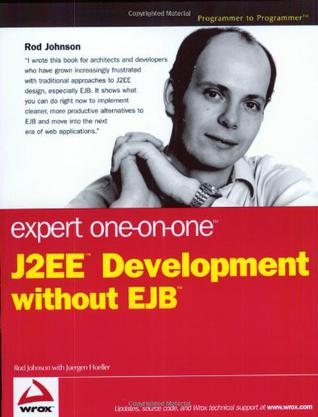
\includegraphics[width=0.3\textwidth]{../expert_one_on_one.jpg}
    \end{itemize}
  }

  \bgroup
  \usenavigationsymbolstemplate{}
  \setbeamercolor{background canvas}{bg=black}
  \frame[plain]{
    \begin{center}
      
\includegraphics[width=0.8\textwidth]{../continue.jpg}
    \end{center}
  }
  \egroup

\end{CJK}
\end{document}
